\documentclass{article}
\usepackage[utf8]{inputenc}
\usepackage{pgfplots}

\pgfplotsset{compat=1.3, xlabel=$x$,ylabel=$y$,zlabel=$z$}

\begin{document}

\section*{Figura 3, $\Delta x=\Delta y=\frac{2}{3}$}

\pgfplotsset{width=9cm}

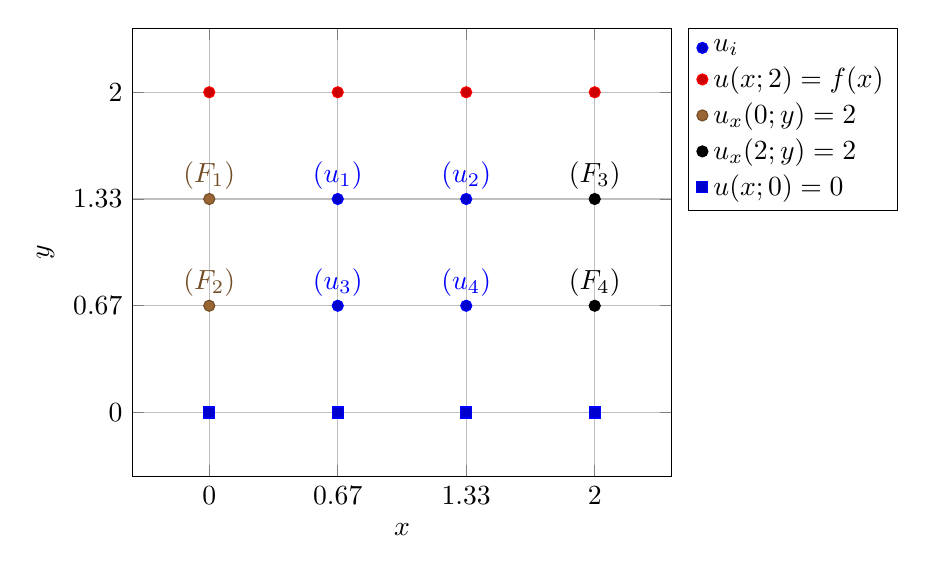
\begin{tikzpicture}
\begin{axis}[grid,xtick distance=2/3,ytick distance=2/3,legend cell align=left,
legend pos=outer north east,nodes near coords,enlargelimits=0.2]

\addplot+[only marks,
point meta=explicit symbolic]
coordinates {
    (2/3,2/3) [($u_3$)]
    (4/3,2/3) [($u_4$)]

    (2/3,4/3) [($u_1$)]
    (4/3,4/3) [($u_2$)]
};
\addplot+[only marks,mark=*,
point meta=explicit symbolic]
coordinates{
    (0,2)
    (2/3,2)
    (4/3,2)
    (2,2)
};

\addplot+[only marks,mark=*,
point meta=explicit symbolic]
coordinates{
    (0,4/3) [($F_1$)]
    (0,2/3) [($F_2$)]
};
\addplot+[only marks,mark=*,
point meta=explicit symbolic]
coordinates{
    (2,4/3) [($F_3$)]
    (2,2/3) [($F_4$)]
};
\addplot+[only marks,mark=square*,
point meta=explicit symbolic]
coordinates{
    (0,0)
    (2/3,0)
    (4/3,0)
    (2,0)
};
\legend{$u_i$,$u(x;2)=f(x)$,$u_x(0;y)=2$,$u_x(2;y)=2$,$u(x;0)=0$}
\end{axis}
\end{tikzpicture}

\pgfplotsset{width=12cm,view={35}{45},xtick distance=2/3,ytick distance=2/3}
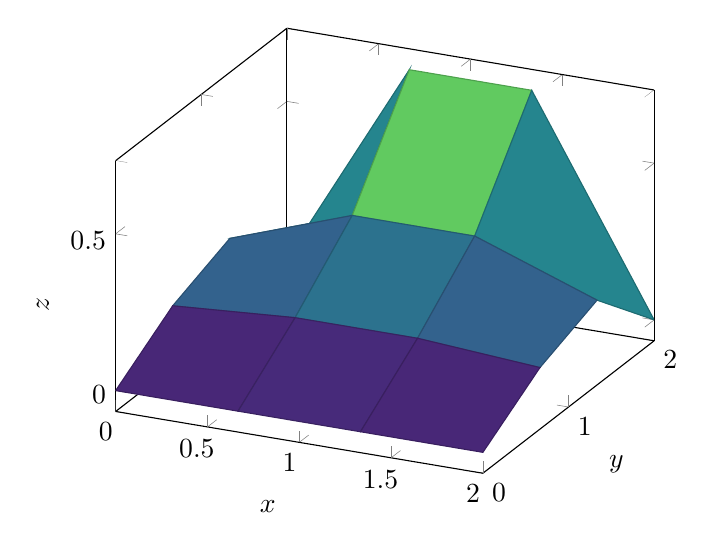
\begin{tikzpicture}
\begin{axis}[colormap/viridis]
\addplot3[surf]coordinates{
(0,0,0) (2/3,0,0) (4/3,0,0) (2,0,0)

(0,2/3,7/54) (2/3,2/3,17/108) (4/3,2/3,17/108) (2,2/3,7/54)

(0,4/3,11/54) (2/3,4/3,37/108) (4/3,4/3,37/108) (2,4/3,11/54)

(0,2,0) (2/3,2,2/3) (4/3,2,2/3) (2,2,0)
};
\end{axis}
\end{tikzpicture}

\pgfplotsset{width=12cm,view={120}{65}}
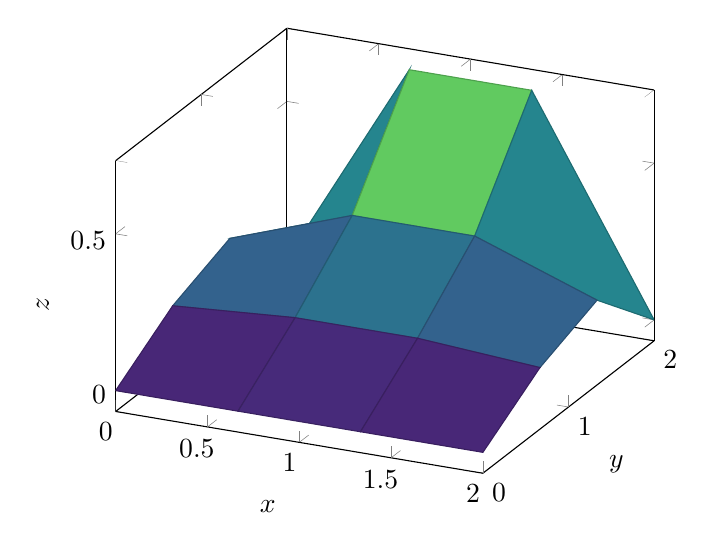
\begin{tikzpicture}
\begin{axis}[colormap/viridis]
\addplot3[surf]coordinates{
(0,0,0) (2/3,0,0) (4/3,0,0) (2,0,0)

(0,2/3,7/54) (2/3,2/3,17/108) (4/3,2/3,17/108) (2,2/3,7/54)

(0,4/3,11/54) (2/3,4/3,37/108) (4/3,4/3,37/108) (2,4/3,11/54)

(0,2,0) (2/3,2,2/3) (4/3,2,2/3) (2,2,0)
};
\end{axis}
\end{tikzpicture}

\section*{Figura 4, $\Delta x=\Delta y=\frac{1}{2}$}
\pgfplotsset{width=8cm}
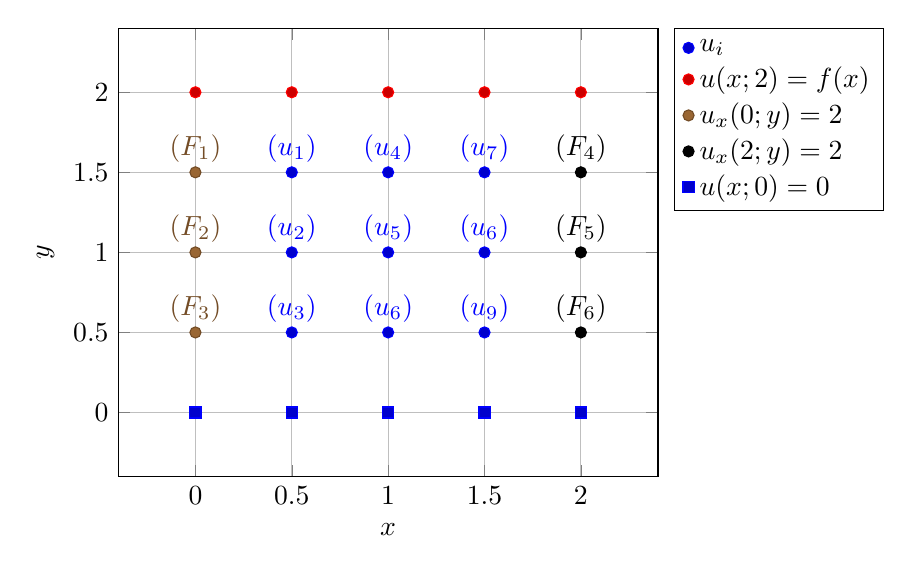
\begin{tikzpicture}
\begin{axis}[grid,legend cell align=left,
legend pos=outer north east,nodes near coords,enlargelimits=0.2,xtick distance=0.5,ytick distance=0.5]
\addplot+[only marks,
point meta=explicit symbolic]
coordinates {
    (0.5,0.5) [($u_3$)]
    (1,0.5) [($u_6$)]
    (1.5,0.5) [($u_9$)]

    (0.5,1) [($u_2$)]
    (1,1) [($u_5$)]
    (1.5,1) [($u_6$)]

    (0.5,1.5) [($u_1$)]
    (1,1.5) [($u_4$)]
    (1.5,1.5) [($u_7$)]
};
\addplot+[only marks,mark=*,
point meta=explicit symbolic]
coordinates{
    (0,2)
    (0.5,2)
    (1,2)
    (1.5,2)
    (2,2)
};
\addplot+[only marks,mark=*,
point meta=explicit symbolic]
coordinates{
    (0,1.5) [($F_1$)]
    (0,1) [($F_2$)]
    (0,0.5) [($F_3$)]
};
\addplot+[only marks,mark=*,
point meta=explicit symbolic]
coordinates{
    (2,1.5) [($F_4$)]
    (2,1) [($F_5$)]
    (2,0.5) [($F_6$)]
};
\addplot+[only marks,mark=square*,
point meta=explicit symbolic]
coordinates{
    (0,0)
    (0.5,0)
    (1,0)
    (1.5,0)
    (2,0)
};
\legend{$u_i$,$u(x;2)=f(x)$,$u_x(0;y)=2$,$u_x(2;y)=2$,$u(x;0)=0$}
\end{axis}
\end{tikzpicture}

\pgfplotsset{width=12cm,view={35}{45}}

\begin{tikzpicture}
\begin{axis}[colormap/viridis]
\addplot3[surf]table{H2.txt};
\end{axis}
\end{tikzpicture}

\pgfplotsset{width=12cm,view={120}{65}}

\begin{tikzpicture}
\begin{axis}[colormap/viridis]
\addplot3[surf]table{H2.txt};
\end{axis}
\end{tikzpicture}

\pgfplotsset{width=12cm,view={35}{45},xtick distance=0.25,ytick distance=0.25}

\begin{tikzpicture}
\begin{axis}[colormap/viridis]
\addplot3[surf]table{H3.txt};
\end{axis}
\end{tikzpicture}

\pgfplotsset{width=12cm,compat=1.3,view={120}{65},xtick distance=0.25,ytick distance=0.25}

\begin{tikzpicture}
\begin{axis}[colormap/viridis]
\addplot3[surf]table{H3.txt};
\end{axis}
\end{tikzpicture}

\end{document}
